\documentclass[notitlepage,12pt,a4paper]{report}
\usepackage[utf8]{inputenc}
\usepackage[russian]{babel}
\usepackage[margin=2cm]{geometry}

\usepackage[vectors,derivative,root]{hedmaths}
\usepackage[column]{hedfeatures}

\usepackage{pscyr}

\usepackage{graphicx}
\graphicspath{{images/}}

\usepackage[usenames,dvipsnames]{color}
\usepackage[colorlinks,linkcolor=black,citecolor=black,urlcolor=Blue]{hyperref}

\newcommand{\E}{\mathcal{E}}
\newcommand{\h}{\mathcal{H}}

\addto\captionsrussian{\renewcommand\bibname{Ссылки}}
\usepackage{cite}

\makeatletter   
\renewcommand\@biblabel[1]{\textsuperscript{#1}}

\def\@cite#1#2{\leavevmode\cite@adjust%
  \textsuperscript{#1\if@tempswa\@safe@activesfalse\citemid{#2}\fi
  \spacefactor\@m
  }
 \@restore@auxhandle}

\renewcommand{\@makechapterhead}[1]{%
  {\parindent \z@ \raggedright \normalfont
    \ifnum \c@secnumdepth >\m@ne
        \Large\bfseries \@chapapp\space \thechapter.\space
    \fi
    \Large \bfseries #1\par\nobreak
    \vskip 3ex
  }}
\renewcommand{\@makeschapterhead}[1]{%
  {\parindent \z@ \raggedright
    \normalfont
    \interlinepenalty\@M
    \Large \bfseries  #1\par\nobreak
    \vskip 3ex
  }}

\renewcommand\section{\@startsection      {section}{1}{\z@}{3ex}{3ex}%
                                          {\normalfont\large\bfseries}}
\renewcommand\subsection{\@startsection   {subsection}{2}{\z@}{2ex}{2ex}%
                                          {\normalfont\normalsize\bfseries}}
\renewcommand\subsubsection{\@startsection{subsubsection}{3}{\z@}{1.5ex}{1.5ex}%
                                          {\normalfont\normalsize}}
\renewcommand\paragraph{\@startsection    {paragraph}{4}{\z@}{1ex}{-1em}
                                          {\normalfont\normalsize}}
\renewcommand\subparagraph{\@startsection {subparagraph}{5}{\parindent}{1ex}{-1em}%
                                          {\normalfont\normalsize}}
\makeatother

\begin{document}
  
  \begin{center}
    In contrast to single-component superconductors, which are described at the
    level of Ginzburg-Landau theory by a single parameter \( \kappa \) and are
    divided in type-I \( \kappa < 1/\sqrt{2} \) and type-II
    \( \kappa > 1/\sqrt{2} \) classes, two-component systems in general possess
    three fundamental length scales and have been shown to possess a separate
    <<type-1,5>> superconducting state\cite{bib:1,bib:2}
. In that state, as a consequence of
the extra fundamental length scale, vortices attract one another at long range but repel at shorter
ranges, and therefore should form clusters in low magnetic fields. In this work we investigate the
appearance of type-1.5 superconductivity and the interpretation of the fundamental length scales
in the case of two active bands with substantial interband couplings such as intrinsic Josephson
coupling, mixed gradient coupling and density-density interactions. We show that in the presence
of substantial intercomponent interactions of the above types the system supports type-1.5 super-
conductivity with fundamental length scales being associated with the mass of the gauge field and
two masses of normal modes represented by mixed combinations of the density fields.
  \end{center}
  
  \chapter{Введение}
\label{ch:1}

According to Ginzburg-Landau theory, a conventional superconductor near 
\( T \) c is described by a single complex order parameter field. The physics 
of these systems is governed by two fundamental length scales, the magnetic
field penetration depth \( \lambda \) and the coherence length \( \xi \), and
the ratio \( \kappa \) of these determines the response to an external
field, sorting them into two categories as follows; type-I when 
\( \kappa < 1/\sqrt{2} \) and type-II when \( \kappa > 1/\sqrt{2} \)
\footnotemark[3].

Type-I superconductors expel weak magnetic fields, while strong fields give 
rise to formation of macroscopic normal domains with magnetic flux 4. The 
response of type-II superconductors is completely different; below some 
critical value \( H_{c1} \), the field is expelled. Above this value a 
superconductor forms a lattice or a liquid of vortices that have a 
supercurrent circulating around a normal core and carry magnetic flux through 
the system. Finally, at a higher second critical value, \( H_{c2} \) 
superconductivity is destroyed. 

These different responses are usually viewed as consequences of the vortex 
interaction in these systems, the energy cost of a boundary between 
superconducting and normal states and the thermodynamic stability of vortex 
excitations. In a type-II superconductor the energy cost of a boundary between 
the normal and the superconducting state is negative, while the interaction 
between vortices is repulsive 3. This leads to a formation of stable vortex 
lattices and liquids. In type-I superconductors the situation is the opposite; 
the vortex interaction is attractive (thus making them unstable against 
collapse into one large vortex), while the boundary energy between normal and 
superconducting states is positive. From a thermodynamic point of view the 
principal difference between type-I and type-II states is the following: (i) 
In type-II superconductors the external magnetic field strength required to 
make formation of vortex excitations energetically preferred, \( H_{c1} \), 
is smaller than the thermodynamical magnetic field \( H_{ct} \) (the field 
whose energy density is equal to the condensation energy of a superconductor, 
i.e. the field at which the uniform superconducting state becomes 
thermodynamically unstable); (ii) In type-I superconductors the field strength 
required to create a vortex excitation is larger than the thermodynamical 
critical magnetic field i.e. vortices cannot form. One can distinguish also a 
special "zero measure" boundary case where \( \kappa \) has a critical value 
exactly at the type-I/type-II boundary, which in the most common GL model 
parameterization corresponds to \( \kappa = 1/\sqrt{2} \). In that case 
vortices do not interact 5 in the Ginzburg-Landau theory. 

The above circumstances result in a situation where, in a strong external 
magnetic field, type-I superconductors usually have a tendency to minimize 
boundary energy between the normal and superconducting states, leading to a 
formation of large inclusions of normal phase which frequently have laminar 
structure \( ^4 \). 

Recently there has been increased interest in superconductors with several 
superconducting components. The main situations where multiple superconducting 
components arise are (i) multiband superconductors 6 - 11 , (ii) mixtures of 
independently conserved condensates such as the projected superconductivity 
in metallic hydrogen and hydrogen rich alloys 12–14 and (iii) superconductors 
with other than s-wave pairing symmetries. In this work we focus on the cases 
(i) and (ii). The principal difference between the cases (i) and (ii) is the 
absence of the inter-component Josephson coupling in case (ii). 

In two-band superconductors (i) the superconducting components originate from 
electronic Cooper pairing in different bands 6. Therefore these condensates 
could not a priori be expected to be independently conserved. This, at the 
level of effective models should manifest itself in a rather generic presence 
of intercomponent Josephson coupling. 

In the case (ii) two superconducting components were predicted to originate 
from electronic and protonic Cooper pairing in metallic hydrogen or 
hydrogen-rich alloys. In the projected liquid metallic deuteriumor 
deuterium-rich alloys, electronic superconductivity was predicted to coexist 
at ultra high pressures with deuteronic condensation 12–14 . Because electrons 
cannot be converted to protons or deuterons the condensates are independently 
conserved, and therefore in the effective model intercomponent Josephson 
coupling is forbidden on symmetry grounds. These states are currently a 
subject of a renewed experimental pursuit. They are expected to arise at high 
but experimentally accessible pressures (\( \approx 400 \)~GPa). Current 
static compression experiments achieve pressures of \( \approx 350 \)~GPa 
with pressures of an order of 1TPa being anticipated in diamond anvil cell 
experiments due to the recent availability of ultra hard diamonds. Similar 
two-charged component models were discussed in the context of the physics of 
neutron stars where they represent coexistent protonic and 
\( \Sigma^\text{--} \)-hyperon Cooper pairs in the neutron star 
interior\( ^{15} \). 

This wide variety of systems raises the need to understand and classify the 
possible magnetic responses of multicomponent superconductors. It was 
discussed recently that in multicomponent systems the magnetic response is 
much more complex than in ordinary systems, and that the type-I/type-II 
dichotomy is not sufficient for classification. Rather, in a wide range of 
parameters, as a consequence of the existence of three fundamental length 
scales, there is a separate superconducting regime where vortices have 
long-range attractive, short-range repulsive interaction and form vortex 
clusters immersed in domains of two-component Meissner state 1,2. Recent 
experimental works 16,17 have put forward the suggestion that this state is 
realized in the two-band material \( MgB_2 \), which sparked growing interest 
in this topic. In particular questions were raised over whether this 
"type-1.5" superconducting regime (as it was termed by Moshchalkov et 
al\( ^{16} \), for recent works see 18 ) is possible even in principle in the 
case of various non vanishing couplings (e.g. intrinsic Josephson coupling, 
mixed gradient couplings etc) between superconducting components in different 
bands. 

In this work we report a study of the appearance of type-1.5 superconductivity 
especially focusing on the case of multiband superconductivity, demonstrating 
the persistence of this type of superconductivity in the presence of various 
kinds of intercomponent couplings (such as interband Josephson coupling, mixed 
gradient coupling, density-density, and other kinds coupling).

\section{Сверхпроводимость типа 1,5}
\label{sec:1-1}

The possibility of a new type of superconductivity, distinct from the type-I 
and type-II in multicomponent systems 1,2 is based on the following 
considerations. In principle the boundary problem in the Ginzburg-Landau type 
of equations in the presence of phase winding is not, from a rigorous point of 
view, reducible to a one-dimensional problem in general. Furthermore, as 
discussed in 1,2 , in general in two-component models there are three 
fundamental length scales which renders the

\begin{figure}[h!]
  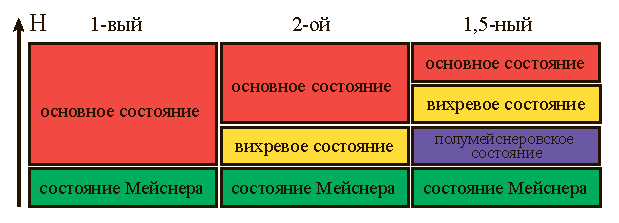
\includegraphics[width=.5\textwidth]{1-01}
  \caption{A comparison of the magnetic phase diagrams of
    clean bulk type-I,type-II and type-1.5 superconductors at
    zero temperature. The semi-Meissner state is a macroscopic
    phase separation into two-component Meissner state and vortex
    clusters where one of the density modes is suppressed by
    core overlaps}
\end{figure}


model impossible to parametrize in terms of a single dimensionless parameter 
\( \kappa \). In the case where the condensates are not coupled by interband 
Josephson coupling but only by the vector potential these length scales are
the two independent coherence lengths (set by the inverse masses of the 
corresponding scalar density fields) and magnetic field penetration length 
(set by the inverse mass acquired by the gauge field). In contrast, in the 
case where the condensates are coupled by inter-band Josephson terms, one 
cannot distinguish independent coherence lengths attributed to different 
condensates. Nonetheless, in this case the density variations can also possess 
two fundamental length scales 2 , in contrast to single-component theories. 
We elaborate on this fact below. In 1,2 vortex solutions in two-component 
theories were found which have non-monotonic vortex inter-action, with a long 
range attractive part determined by a dominant density-density interaction and 
a short range repulsive part produced by current-current and electro-magnetic 
interactions. An important circumstance which was demonstrated was that these 
vortices are thermodynamically stable in spite of the existence of the 
attractive tail in the interaction.

A non-monotonic intervortex interaction potential should result in the 
formation of vortex clusters in low magnetic field immersed into the 
vortexless areas, a state referred to in 1 as the "semi-Meissner state". 
Figure 1 shows the schematic phase diagram of a type-1.5 superconductor.

If the vortices form clusters one cannot use the usual one-dimensional 
argument concerning the energy of superconductor-to-normal state boundary to 
classify the magnetic response of the system. First of all, the energy per 
vortex in such a case depends on whether a vortex is placed in a cluster or 
not: i.e. formation of a single isolated vortex might be energetically 
unfavorable, while formation of vortex clusters is favorable, because in a 
cluster where vortices are placed in a minimum of the interaction potential, 
the energy per flux quantum issmaller than that for an isolated vortex 
(thermodynamically the nonmonotonic two-vortex interaction potential predicts 
that the smallest energy per flux quantum will be in the case of a uniform 
lattice with spacing equal to the minimum of two-body intervortex potential).

Thus, besides the energy of a vortex in a cluster, there appears an additional 
energy characteristic associated with the boundary of a cluster. In other 
words, in this situation, to determine the magnetic response of a system it is 
not sufficient to study the one-dimensional boundary problem nor the 
single-vortex problem, in contrast to single component systems. Moreover, in a 
cluster the system tends to minimize the boundary energy of a cluster 
(similarly to type-I behavior), while breaking into a lattice of one-quantum 
vortices inside the cluster (similarly to type-II systems with negative 
interface energy). Thus, in an increased magnetic field the vortices form via 
a first order phase transition. A magnetic phase distinct from the vortex and 
Meissner states which then arises is a macroscopic phase separation into 
domains of two-component Meissner state and vortex clusters where one of the 
density modes is suppressed by core overlap. We summarize the basic properties 
of type-I, type-II and type-1.5 regimes in the table I.

The existence of thermodynamically stable type-1.5 superconducting regimes 
ultimately depends on the existence of a nonmonotonic intervortex interaction 
potential. It is an important question how generic this effect is. In this 
work we mainly focus on multiband realizations of multicomponent 
superconductivity and investigate the effects of interband Josephson coupling, 
mixed gradient coupling, and density-density coupling terms on vortex 
interactions in two band superconductors. We show that (i) when these 
couplings are present, the system still can possess three fundamental length 
scales, in contrast to the two length scales in the usual single-component GL 
theory; (ii) non-monotonic interaction is possible in a wide parameter range 
in these models.

The structure of this paper is as follows: In section II we introduce the 
model.In section III we present a linear theory of asymptotics of the vortex 
fields in a superconductor with two bands with various interband couplings.

We begin section III by demonstrating that for a general form of the effective 
potential in a two-band (or more generally two-gap) Ginzburg-Landau free 
energy, the linear theory gives, under quite general conditions, two 
fundamental length scales of the variations of the densities. From the 
linearized theory we calculate the long-range intervortex interaction 
potentials using the two-component generalization of the point-vortex method 
19 and show how the non-monotonic intervortex interaction potential arise from 
the interplay of two fundamental length scales of the superfluid density 
variations and the magnetic field penetration length. The central point of 
this part is how the fundamental length scales are defined in the presence of 
interband coupling as well as the occurrence of "mode mixing". Next we move to 
quantitatively study the effects of several kinds of intercomponent couplings 
which quite generically arise in two-component theories.

In section III (d) we demonstrate that that mixed gradient coupling can lead 
under certain conditions to an increase in the disparity of the characteristic 
scales of the density variations.

In Section IV we present a large scale numerical study of the full nonlinear 
problem of the interaction between a pair of vortices.
 \newpage
  \chapter{Модель}
\label{ch:2}

\section{Функционал свободной энергии}
\label{sec:2-1}

Тип 1.5 изучается с помощью следующей двухкомпонентного функционала 
свободной энергии Гинзбурга-Ландау (ТГЛ):
\begin{align}
	F = \frac{1}{2}(D\psi_1)(D\psi_1)^* + \frac{1}{2}(D\psi_2)(D\psi_2)^* - 
		\nu Re\left( (D\psi_1)(D\psi_2)^* \right) + 
		\frac{1}{2}\left(\nabla\times\vec{A}\right)^2 + F_p
	\label{eq:1}
\end{align}

Здесь \( D = \nabla + ie\vec{A} \) и \( \psi_a = |\psi_a|e^{i\theta_a} \), 
\( a = 1,2 \), представляет собой две сверхтекучих компоненты, которые в 
двухщелевом сверхпроводнике соответствуют двум сверхтекучим плотностям в 
в различных диапазонах. Слагаемое \( F_p \) может содержать в нашем 
анализе произвольный набор не градиентных членов.

Особая форма двухкомпонентной модели ГЛ точно 
выведенная\cite{bib:8,bib:9,bib:10} для двухщелевых сверхпроводников является:
\begin{align}
	F = & \frac{1}{2}(D\psi_1)(D\psi_1)^* + \frac{1}{2}(D\psi_2)(D\psi_2)^* - 
		\nu Re\left\{ (D\psi_1)(D\psi_2)^* \right\} + 
		\frac{1}{2}\left(\nabla\times\vec{A}\right)^2 + \alpha_1|\psi_1|^2 + 
		\nonumber \\
		& + \frac{1}{2}\beta_1|\psi_1|^4 + \alpha_2|\psi_2|^2 + 
		\frac{1}{2}\beta_2|\psi_2|^4 + \eta_1|\psi_1||\psi_2|
		\cos(\theta_1-\theta_2) + \eta_2|\psi_1|^4|\psi_2|^2
	\label{eq:2}
\end{align}

Первые два слагаемых представляют стандартный градиентный член 
Гинзбурга-Ландау, второе слагаемое представляет смешанные градиентные 
взаимодействия, которые появляются в двухщелевых сверхпроводниках с примесным 
рассеянием \cite{bib:8,bib:9}. Следующее член является плотностью энергии 
магнитного поля, а остальные слагаемые представляют эффективный потенциал. 
Здесь же отметим, что \( \alpha_1 \) и \( \alpha_2 \) могут инвертировать знак 
при различных температурах. Режим где \( \alpha_1 \) положительно, в то время 
\( \alpha_2 \) отрицательно, что соответствует ситуации, когда один из группы 
не имеет собственной сверхпроводимости, но, тем не менее имеет некоторые 
сверхтекучие плотности из-за межзонного туннелирования Джосефсона, которая 
представлена \( \eta|\psi_1||\psi_2|\cos(\theta_1-\theta_2) \) слагаемым. 
Поведения типа 1.5 в этом режиме был исследован в\cite{bib:2}. В этой работе 
мы в основном сосредоточимся на ситуации когда обе зоны являются активными, 
т.е. \( \alpha_{1,2} < 0 \). Для общности добавим слагаемое более высокого 
порядка связи плотность-плотность \( \eta_2|\psi_1|^2|\psi_2|^2 \). Мы также 
рассмотрим случай независимо сохраняющихся конденсатов, где третий и девятый 
члены в \eqref{eq:2} запрещены на основании симметрии, то есть 
\( \nu = \eta_1 = 0 \) (см. также замечание\cite{bib:21}). Эквивалентность 
между нашими единицами и общепринятого даётся в Приложении \ref{ch:A}.

Точно выведенная модель ГЛ \eqref{eq:2} необходимо малость полей 
\( |\psi_a| \). Однако это не требует в принципе от \( \alpha_a \) менять знак 
при той же температуре. Кроме того, как и в случае однокомпонентной теории ГЛ, 
мы ожидаем, что модель \eqref{eq:2} даёт во многих случаях приемлемую картину 
в низкотемпературном режиме. Фактически, наш анализ может в некоторых случаях 
дать качественную картину для случая, когда одно из полей не обладает 
эффективным потенциалом ГЛ-типа, так как режим, где одна из зон в Лондоновском 
приближении (т.е. она не обладает эффективным потенциалом ГЛ, но небольшое ядро 
вихря моделируется резкой границей отсечки) может быть восстановлена из 
нашего анализа, как предельный случай. Как будет ясно ниже из анализа этого 
режима он также поддерживает сверхпроводимость типа 1,5.

\begin{table}[ht]
    \centering
    \begin{tabular}{|C{.18}|C{.22}|C{.22}|C{.35}|}
        \hline
        & однокомпонентный тип I & однокомпонентный тип II & 
        многокомпонентный тип 1.5 \\ \hline

        Масштабная характерная длина & Глубина проникновения \( \lambda \) и 
            длина когерентности \( \xi \) 
            (\( \frac{\lambda}{\xi} < \frac{1}{\sqrt{2}} \)) &
        Глубина проникновения \( \lambda \) и 
            длина когерентности \( \xi \) 
            (\( \frac{\lambda}{\xi} > \frac{1}{\sqrt{2}} \)) &
        Две характеристические вариации плостностей масштабных величин 
            \( \xi_1, \xi_2 \) и глубина проникновения \( \lambda \), 
            немонотонное взаимодействие вихря происходит в этих системах, как 
            правило, когда \( \xi_1 < \sqrt{2}\lambda < \xi_2 \) \\ \hline

        Межвихревое взаимодействие & Притягивающий & Отталкивающий & 
            Притягивающий на больших расстояниях и отталкивающий на коротких 
        \\ \hline

        Энергия сверхпроводников/граница фаз & Положительный & Отрицательный &
            При довольно общих условиях отрицательной энергии сверхпроводника / 
            границы раздела внутри вихревого скопления, но положительна вне (!!).

        \\ \hline

        Магнитное поле, необходимое для образования вихря & Больше чем 
            критическое термодинамическое магнитное поле & Меньше чем 
            критическое термодинамическое магнитное поле &
        В различных случаях либо (i) меньше, чем критическое термодинамическое 
            магнитное поле или (ii) больше, чем критическое термодинамическое
            магнитное поле для одиночного вихря, но меньше критического 
            магнитного поля для вихревого образования некоторого критического 
            размера.

        \\ \hline

        Этапы внешнего магнитного поля & (i) Эффект Мейснера для слабых полей; 
            (ii) Макроскопически большее нормальное состояние в больших полях. 
            Фазовый переход первого рода между сверхпроводящим (Мейснер) и 
            нормальным состоянием & (i) Эффект Мейснера для слабых полей; (ii) 
            вихревые решётки/жидкости при больших полях. Фазовые переходы 
            второго рода между состоянием Мейснера и вихревым, а также 
            между вихревым и нормальным. & (i) Эффект Мейснера для слабых 
            полей. (ii) полумейсснеровское состояние": вихревые образования 
            сосуществуют с областью Мейснера на промежуточных полях. (iii) 
            Вихревые решётки/жидкости при больших полях. Вихревая форма путём 
            фазового перехода первого рода. Переход от вихревого состояния в 
            нормальное состояния является переходом второго рода (!!).
        \\ \hline

        Энергия \( E(N) \) или N-квантовые аксиально-симметричные вихревые 
            решения(!) & \( \frac{E(N)}{N} < \frac{E(N-1)}{N-1} \) для всех 
            \( N \). Вихри сливаются в единый \( N \)-квантовой мегавихрь &
        \( \frac{E(N)}{N} > \frac{E(N-1)}{N-1} \) для всех \( N \). 
            \( N \)-квантовый вихрь распадается на \( N \) бесконечно 
            разделенных одноквантовых вихрей & Здесь характеристическое число 
            \( N \) такое, что \( \frac{E(N)}{N} < \frac{E(N-1)}{N-1} \) для 
            \( N < N_c \), тогда как 
            \( \frac{E(N)}{N} > \frac{E(N-1)}{N-1} \) для \( N > N_c \). 
            N-квантовые вихри распадаются на вихревые образования.
        \\ \hline

    \end{tabular}
    \caption{Основные характеристики чистых сверхпроводников первого, второго и 
        1,5 рода. Здесь указаны наиболее распространённые единицы измерения 
        используемые в теории ГЛ, которые подразделяются на первый и второй 
        род в однокомпонентной теории параметром \( \kappa_c = 1/\sqrt{2} \)}
\end{table}

\section{Основные свойства вихревых возбуждений}
\label{sec:2-2}

Единственные вихревые решения модели \eqref{eq:2}, которые имеют конечную 
энергию на единицу длины являются целыми N-поточными квантовыми вихрями, 
которые имеют следующие фазовые обороты вдоль контура \( l \) вокруг вихря: 
\( \oint\limits_l \nabla\theta_l = 2\pi N \), 
\( \oint\limits_l \nabla\theta_l = 2\pi N \). Вихрь с разным фазовым закруткой 
несёт дробное число, кратное кванту магнитного потока и обладающий
расходящейся энергией с размером системы. Решения подробно исследованы в
\cite{bib:22}.

В дальнейшем мы исследуем только целочисленные вихревые решения, которые 
являются энергетически выгодными объектами производимыми с помощью внешнего 
поля в объёмном сверхпроводнике. \newpage
  \chapter{Вихревая асимптотика}
\label{ch:3}

Ключом к пониманию взаимодействия хорошо разделенных вихрей является анализ  
больших \( r \) асимптотического вихревого решения. Мы проанализируем эту 
проблему в контексте общей двухкомпонентной модели ГЛ, чья свободная энергия 
принимает форму
\begin{equation}
    F = \frac{1}{2}\left( D_i \psi_1 \right)^{*} D_i \psi_1 + 
        \frac{1}{2}\left( D_i \psi_2 \right)^{*} D_i \psi_2 + 
        \frac{1}{2}\left( \partial_1 A_2 - \partial_2 A_1 \right)^2 + F_p
    \label{eq:3}
\end{equation}
где \( F_p \) содержит все не-градиентные члены (в частности, но не 
ограничиваясь, джозефсоновским и плотность-плотность членами взаимодействия). 
Эта свободная энергия соответствует \eqref{eq:2} в случае \( \nu = 0 \). 
We will show in section IIID how to handle mixed gradient terms. The precise 
form of \( F_p \) is not crucial for our analysis in this section. By gauge 
invariance, it can depend on the condensates only via \( |\psi_1|, |\psi_2| \) 
and (if the condensates are not independently conserved) on 
\( \theta_1 - \theta_2 \). We will assume that \( F_p \) takes its minimum 
value (which we normalize to be 0) when 
\( |\psi_1| = u_1 > 0, |\psi_2| = u_2 > 0 \) and 
\( \theta_1 - \theta_2 = 0 \). So, either there is no phase coupling 
(\( F_p \) is independent of \( \theta_1 - \theta_2 \)) and the choice of 
\( \theta_1 - \theta_2 = 0 \) is arbitrary, or the phase coupling is such as 
to encourage phase locking. (Note that the case of phase anti-locked fields 
can trivially be recovered from our analysis by mapping 
\( \psi_2 \mapsto -\psi_1 \)).

The field equations are obtained from \( F \) by demanding that the total 
free energy \( E = \int F dx_1 dx_2 \) is stationary with respect to all 
variations of \( \psi_1, \psi_2 \) and \( A_i \). A routine calculation yields 
\begin{gather}
    D_i D_i \psi_a = 2\pder{F_p}{\psi_a^{*}}
    \label{eq:4} \\
    \partial_i \left( \partial_i A_j - \partial_j A_i \right) = 
        e\sum\limits_{a=1}^{2}\Im\left( \psi_a^* D_j \psi_a \right)
    \label{eq:5}
\end{gather}
This triple of coupled nonlinear partial differential equations supports 
solutions of the form
\begin{gather}
    \psi_a = f_a(r)e^{i\theta} \nonumber \\
    (A_1, A_2) = \frac{a(r)}{r}(-\sin\theta, \cos\theta)
    label{eq:6}
\end{gather}
where \( f_1, f_2, a \) are real profile functions. Note that in some cases 
mixed gradient terms favour non-axially symmetric solutions. In this section 
we consider only axially symmetric vortices. Fields within the above ansatz 
satisfy the field equations if and only if the profile functions 
\( f_1(r), f_2(r), a(r) \) satisfy the coupled ordinary differential equation 
system
\begin{gather}
    f''_a + \frac{1}{r} f'_a - \frac{1}{r^2}(1+ea)^2 f_a = 
        \left. \pder{F_p}{|\psi_a|} \right|_{(u_1, u_2, 0)}
    \label{eq:7} \\
    a'' - \frac{1}{r} a' - e(1+ea)(f_1^2+f_2^2) = 0
    \label{eq:8}
\end{gather}
The solution we require, the vortex, has boundary behaviour 
\( f_a(r) \rightarrow u_a \), \( a(r) \rightarrow -1/e \) as 
\( r \rightarrow \infty \). So, for large \( r \), the quantities 
\begin{equation}
    \epsilon_a(r) = f_a(r) - u_a, \quad
    \alpha(r) = a(r) + \frac{1}{e}
    \label{eq:9}
\end{equation}
are small and so should, to leading order, satisfy the linearization of 
\eqref{eq:7},\eqref{eq:8} about \( (u_1, u_2, -1/e) \). That is, at large 
\( r \),
\begin{gather}
    \epsilon''_a + \frac{1}{r} \epsilon'_a = \sum\limits_{b=1}^{2}
        \mathcal{H}_{ab} \epsilon_b
    \label{eq:10} \\
    \alpha'' - \frac{1}{r} \alpha' - e^2(u_1^2 + u_2^2 )\alpha = 0
    \label{eq:11}
\end{gather}
where \( \mathcal{H} \) is the Hessian matrix of 
\( F_p(|\psi_1|, |\psi_2|, 0) \) about its minimum 
\begin{equation}
    \mathcal{H}_{ab} = \left. \pcder{F_p}{|\psi_a|}{|\psi_b|} 
        \right|_{(u_1, u_2, 0)}
    \label{eq:12}
\end{equation}
So \( \alpha \) decouples from \( \epsilon_1, \epsilon_2\) asymptotically, and 
we see immediately that
\begin{equation}
    \alpha(r) = q_0 r K_1(\mu_A r), \quad
    \mu_a = e\sqrt{u_1^2 + u_2^2}
    \label{eq:13}
\end{equation}
where \( K_n \) denotes the nth modified Bessel’s function of the second 
kind\( ^{23} \), and \( q_0 \) is an unknown real constant. Hence, at large,
\begin{equation}
    \vec{A} \sim \left( -\frac{1}{er} + q_0 K_1(\mu_A r) \right)
        (-\sin\theta, \cos\theta)
    \label{eq:14}
\end{equation}
Since, for all \( n \), 
\begin{equation}
    K_n(s) \sim \sqrt{\frac{\pi}{2s}}e^{-s} \text{ as } s \rightarrow \infty
    \label{eq:15}
\end{equation}
it follows that the magnetic field decays exponentially as a function of 
\( r \), with length scale (penetration depth)
\begin{equation}
    \lambda \equiv \frac{1}{\mu_A} = \frac{1}{e\sqrt{u_1^2 + u_2^2}}
    \label{eq:16}
\end{equation}

By contrast, \eqref{eq:10} represents, in general, a coupled pair of ordinary 
differential equations for \( \epsilon_1, \epsilon_2 \). Since 
\( (u_1, u_2, 0 ) \) is a \textit{minimum} of 
\( F_p(|\psi_1|, |\psi_2|, \theta_1 - \theta_2) \), the Hessian matrix is a 
\textit{positive definite} symmetric \( 2\times2 \) real matrix. Hence its 
eigenvalues, \( \mu_1^2, \mu_2^2\) say, are real and positive, and its 
eigenvectors, \( v_1, v_2 \) say, form an orthonormal basis for 
\( \mathbb{R} \). Expanding in the basis \( v_1, v_2 \)
\begin{equation}
    \epsilon(r) = \chi_1(r) v_1 + \chi_2(r) v_2
    \label{eq:17}
\end{equation}
we see that \( \chi_1, \chi_2 \) satisfy the uncoupled pair of ordinary 
differential equations
\begin{equation}
    \chi''_a + \frac{1}{r}\chi'_a = \mu_a^2 \chi_a
    \label{eq:18}
\end{equation}
whence 
\begin{equation}
    \chi_a(r) = q_a K_0(\mu_a r)
    \label{eq:19}
\end{equation}
for some (unknown) constants \( q_1, q_2 \). Since \( v_1, v_2 \) are 
orthonormal, there is an angle \( \Theta \), which we call the \emph{mixing 
angle}, such that the eigenvectors of \( \mathcal{H} \) are
\begin{equation}
    v_1 = \left( \begin{array}{c}
        \cos\Theta \\
        \sin\Theta
    \end{array} \right), \quad
    v_2 = \left( \begin{array}{c}
        -\sin\Theta \\
        \cos\Theta
    \end{array} \right)
    \label{eq:20}
\end{equation}
Hence, at large \( r \) the density fields behave as
\begin{gather}
    \psi_1 \sim \left[ u_1 + q_1\cos\Theta K_0(\mu_1 r) - 
        q_2\sin\Theta K_0(\mu_2 r) \right]e^{i\theta} \nonumber \\
    \psi_2 \sim \left[ u_2 + q_1\sin\Theta K_0(\mu_1 r) - 
        q_2\cos\Theta K_0(\mu_2 r) \right]e^{i\theta}
    \label{eq:21}
\end{gather}
where, once again, \( K_0 \) is a Bessel function.

From this analysis it follows that:
\begin{enumerate}
    \item In general there are three fundamental length scales in the problem 
        (in contrast to the two length scales of one-component Ginzburg-Landau 
        theory) which manifest themselves in the vortex asymptotics, namely 
        \( 1/\mu_A, 1/\mu_1 \) and \( 1/\mu_2 \).
    \item These are constructed from the vacuum expectation values \( u_a \) 
        of \( |\psi_a| \) (in the case of \( 1/\mu_A \)) and from the 
        eigenvalues of \( \mathcal{H} \), the Hessian matrix of \( F_p \) 
        about the vacuum (i.e. the ground state).
    \item \( 1/\mu_{A} \) can be interpreted as the London penetration length 
        of the magnetic field.
    \item However, unless the mixing angle \( \Theta \) is a multiple of 
        \( \pi/2, 1/\mu_1 \) and \( 1/\mu_2 \) cannot be interpreted as the 
        coherence lengths of \( \psi_1, \psi_2 \) in the usual sense. This is 
        because the normal modes of the field theory close to the vacuum are 
        not \( |\psi_a| - u_a \), but rather
        \[ 
            \chi_1 = (|\psi_1| - u_1)\cos\Theta - (|\psi_2| - u_2)\sin\Theta 
        \]
        \[ 
            \chi_2 = (|\psi_1| - u_1)\sin\Theta - (|\psi_2| - u_2)\cos\Theta 
        \]
        obtained by rotating through the mixing angle \( \Theta \), which is 
        also determined by \( \mathcal{H} \). Therefore in general (e.g. in 
        the presence of intercomponent Josephson coupling) for a one-flux 
        quantum axially symmetric vortex, the recovery of both fields 
        \( \psi_a \) at \emph{very} long range will be according to the same 
        exponential law, set by the smaller of the masses \( \mu_1, \mu_2 \); 
        One should use the representation in terms of the fields 
        \( \chi_{1,2} \) to be handle properly the two length scales 
        associated with the density recovery.
    \item This analysis tells us only about the vortex structure at large 
        \( r \). It gives no direct information on the vortex core, which is 
        important to understand quantitatively the nature of the vortex 
        interactions at intermediate and short distances which will be 
        studied numerically in the section \ref{ch:5}.
\end{enumerate}

Since the gauge field mediates a repulsive force between vortices, while the 
condensate fields mediate an attractive force, it is clear that we can read 
off from the above analysis the condition under which the intervortex force is 
attractive at long range: we require that \( 1/\mu_A \) is \emph{not} the 
longest of the three length scales, or, more explicitly, that (at least) one 
of the eigenvalues of \( \mathcal{H} \) should be less that 
\( \mu_A^2 = e^2(u_1^2 + u_2^2) \). We can predict an explicit formula for 
the long range two-vortex interaction potential, using the point vortex 
formalism\cite{bib:19} (a brief review of the method in given in Appendix C). 
This rests on the observation that, far from its core, the fields of the 
vortex are identical to those of a hypothetical point particle in a linear 
theory with two Klein-Gordon fields (\( \chi_1 \) and \( \chi_2 \) above) of 
mass and a vector field (A) of mass \( \mu_A \). The point particle carries 
scalar monopole charges \( 2\pi q_1 \) and \( 2\pi q_2 \) and a magnetic 
dipole moment \( 2\pi q_0 \). Two such hypothetical particles held distance 
\( r \) apart would experience an interaction potential
\begin{equation}
    V(r) = 2\pi\left[ q_0^2 K_0(\mu_A r) - q_1^2 K_0(\mu_1 r) - 
        q_2^2 K_0(\mu_2 r) \right]
    \label{eq:22}
\end{equation}

This formula reproduces the prediction explained above: the long range 
interaction will be attractive if (at least) one of \( \mu_1, \mu_2 \) is less 
than \( \mu_A \). 

One can ask, retrospectively, whether the approximation of \emph{linearizing} 
in the small quantities \( \alpha(r), \chi_1(r), \chi_2(r) \) is well 
justified. Rigorous analysis of the single component model\cite{bib:20} shows 
that if either of the scalar mode masses, say, exceeds \( 2\mu_A \), then 
quadratic terms in \( \alpha \) become comparable at large \( r \) with linear 
terms in \( \chi_2 \), so that the equation for \( \chi_2 \) should include 
extra terms. In this case, \( \chi_2 \) decays like \( K_0(\mu_A r)^2 \) 
rather than \( K_0(\mu_2 r) \). One should note, however that, unless
\( \mu_1 > 2\mu_A \) also, the leading term in \eqref{eq:21}, decaying like 
\( K_0(\mu_1 r) \), is still correct, and it is only the leading term which 
determines the nature (attractive or repulsive) of the intervortex 
interactions at long range. The case of interest to us is when the long-range 
force is attractive, that is, when at least one of \( \mu_1, \mu_2 \) is 
\emph{less than} \( \mu_A \), so the linearized analysis presented above 
suffices for our purposes.

\section{Симметричная модель \texorpdfstring{$ U(1) \times U(1) $}
  {U(1) x U(1)}}
\label{sec:3-1}

\section{Джозефоновский контакт}
\label{sec:3-2}

\subsection{Сравнение со случаем пассивной второй band (?)}
\label{subsec:3-2-1}

\section{Контакт плотность-плотность (?)}
\label{sec:3-3}

\section{Условия смешанного градиента}
\label{sec:3-4}
 \newpage
  \chapter{Численное решение нелинейной задачи}

\section{Weak Josephson coupling to a passive band}

\section{Effects of Josephson and mixed gradient terms in case of two active
  bands}

\section{Solutions with large disparity in the characteristic length scales}
 \newpage
  \chapter{Выводы}

В этой статье мы представили аналитическое и численное исследование о 
появлении сверхпроводимости типа 1.5 в случае двух зон с различными видами 
существенных межзонных соединений. Во всех случаях, которые мы рассматривали 
мы продемонстрировали, что система обладает тремя основными масштабами длин: 
первая \( 1/\mu_A \) связана с Лондоновской глубиной 
проникновения магнитного поля, в то время как остальные две \( 1/\mu_{1,2} \) 
связаны с характеристической масштабов длин ответственные за изменением 
глубины проникновения поля. В пределе двух конденсатов(?) связанных только с 
электромагнитными масштабными длинами \( 1/\mu_{1,2} \) с независимыми  
длинами когерентности двух полей. Однако мы показали, что введение ненулевой 
Джозефсоновской и density-density связи делают напряжённости полей спадающими 
по экспоненциальному закону при очень больших расстояниях от ядра, в то же 
время система всё ещё обладает двумя основными length scale, которые связаны 
с линейной комбинации напряженности полей повернутыми на <<угол смешивания>>. 
Третья основная масштабная длина в этом режиме является Лондоновской глубиной 
проникновения, и таким образом, двухзонная система со связью позволяет точно 
определить поведения типа-1.5. Далее мы изучали влияние смешанных градиентных 
членов и показали, как тип-1.5 описывается в этом случае. Мы показали, что в 
случае значительного смешанного градиента связи из определения трёх основных 
масштабных длин требуется дополнительные условия, поскольку он даёт режим 
смешивания, который не может быть описан одним углов смешивания. Важно 
отметить нами показанное, что смешанный градиент спаривания может увеличить 
несоответствие характерных масштабных длин изменения плотности. Можно провести 
аналогию между этим механизмом и механизмом качелей в физике нейтрино. Во 
второй части статьи мы представили сравнительное численное исследование 
вихрей типа-1.5 в различных режимах с различными межкомпонентными связями. 
Результаты были продемонстрированы в структуры двухкомпонентной модели 
Гинзбурга-Ландау с локальной электродинамикой. Однако мы ожидаем, что 
описание поведения типа-1.5 подобно присутствию в низких температурных 
режимах и в двухкомпонентных моделях с нелокальной электродинамикой.   

Понятие сверхпроводимости типа-1.5 можно непосредственно обобщить и в 
\( N \)-компонентном случае. Там может иметь место система с  
характерными масштабными длинами 
\( 
	\psi_1, \ldots, \psi_k < \lambda < \psi_{k+1}, \ldots, \psi_N
\) 
и есть термодинамически устойчивые вихри с немонотонным воздействием. 

Кроме многозонных сверхпроводников и сопутствующих электронных и ядерных 
сверхпроводников наша модель может быть реализована в искусственно созданных 
слоистых структурах из материалов типа-I и типа-II, где можно контролировать 
и настраивать межкомпонентную Джозефсоновскую связь.

\emph{Добавленное примечение:} После завершения этой работы, она была проверена в 
детальном расчёте, который не предполагает \( (1-T/T_C \) расширения, что 
модель Гинзбурга-Ландау (2) довольно точно описывает физику вихрей 
двухзонных сверхпроводников в достаточно широком диапазоне параметров и 
температур. \newpage
  \begin{appendix}
    \chapter{Единицы измерения}
\label{ch:A}

В этом разделе мы дадим явное отображение нашего представления модели
ГЛ к более общему виду представленного в учебниках. Рассмотрим модель
Гинзбурга-Ландау в общем представлении
\begin{align}
  F = & \frac{\hbar^2}{2m_1} \abs{\left( \nabla - i\frac{e^*}{\hbar c} A\right)
    \psi_1}^2 + \frac{\hbar^2}{2m_2} \abs{\left( \nabla - i\frac{e^*}{\hbar c}A
    \right) \psi_2}^2 - \nonumber \\
  & - \nu\hbar^2 \Re\left\{ \left( \nabla - i\frac{e^*}{\hbar c}
    \right)\psi_1 \left( \nabla + i\frac{e^*}{\hbar c}A \right)
    \psi^*_2\right\} + \frac{1}{8\pi}\left( \nabla\times A \right)^2 +
    \alpha_1\abs{\psi_1}^2 + \frac{1}{2}\beta_1\abs{\psi_1}^4 + \nonumber \\
  & + \alpha_2\abs{\psi_2}^2 + \frac{1}{2}
    \beta_2\abs{\psi_2}^4 - \eta_1\abs{\psi_1}\abs{\psi_2}
    \cos(\theta_1 - \theta_2) + \eta_2\abs{\psi_1}^2\abs{\psi_2}^2.
    \label{eq:A-1}
\end{align}

Давайте определим обозначенные величины
\begin{gather}
  \tilde{F} = \frac{4\pi}{\hbar^2 c^2}F; \quad
    \tilde{A} = -\frac{A}{\hbar c}; \quad
    \tilde{\psi}_a = \sqrt{\frac{4\pi}{m_a c^2}}\psi_a; \quad
    \tilde{\nu} = \frac{m_1m_2}\nu \nonumber \\
  \tilde{\alpha}_a = \frac{m_a}{\hbar^2}\alpha_a; \quad
    \tilde{\beta}_a = \frac{m^2_a c^2}{4\pi\hbar^2}\beta_a; \quad
    \tilde{\eta}_1 = \frac{\sqrt{m_1 m_2}}{\hbar^2}\eta_1; \quad
    \tilde{\eta}_2 = \frac{m_1 m_2 c^2}{4\pi\hbar^2}\eta_2. \label{eq:A-2}
\end{gather}

Тогда
\begin{align}
  \tilde{F} = & \frac{1}{2}\abs{\left( \nabla + ie^*\tilde{A} \right)
    \tilde{\psi}_2}^2 + \frac{1}{2}\abs{\left( \nabla + ie^*\tilde{A} \right)
    \tilde{\psi}_2}^2 - \tilde{\nu} \Re\left\{ \left( \nabla + ie^*\tilde{A}
    \right)\tilde{\psi}_1 \cdot \left( \nabla + ie^*\tilde{A} \right)
    \tilde{\psi}^*_2 \right\} + \nonumber \\
  & \frac{1}{2}\abs{\nabla\times\tilde{A}}^2 - \tilde{\alpha}_1
    \abs{\tilde{\psi}_1}^2 + \frac{\tilde{\beta}_1}{2}\abs{\tilde{\psi}_1}^2 +
    \tilde{\alpha}_2\abs{\tilde{\psi}_2}^2 +
    \frac{\tilde{\beta}_2}{2}\abs{\tilde{\psi}_2}^2 + \nonumber \\
  & + \tilde{\eta}_1 \abs{\tilde{\psi}_1} \abs{\tilde{\psi}_2}
    \cos(\theta_1 - \theta_2) + \tilde{\eta}_2\abs{\tilde{\psi}_1}^2
    \abs{\tilde{\psi}_2}^2, \label{eq:A-3}
\end{align}
которая, опустив знак тильды, совпадает с представленным \eqref{eq:2} в
данной статье.

На протяжении всей статьи, предполагается, что зона 1 активна, то есть, 
\( \alpha_1 < 0 \). Перепишем уравнение \eqref{eq:2} для \( F \), так, чтобы 
\( \alpha_1 \) была нормирована на \( -1 \) и \( \beta_1 \) нормирована на 
\( 1 \). Это может быть достигнуто следующим образом. Напомним (см. раздел 
\ref{sec:3-1}), что в отсутствии межзонной связи (т.е. когда 
\( \eta_1 = \eta_2 = \nu = 0 \)) конденсат 1 имеет затухание линейного 
масштаба \( 1/\hat{\mu}_1 = (-4\alpha_1)^{-1/2} \). Эта размер обычно
определяется длиной когерентности
\begin{equation}
  \hat{\xi}_1 = \frac{\sqrt{2}}{\hat{\mu}_1} = \frac{1}{\sqrt{-2\alpha_1}}
  \label{eq:A-4}
\end{equation}

Ещё раз подчеркнём, что в присутствии межзонной связи, \( \hat{\xi}_1 \) не
является длиной когерентности конденсата 1. Такое определение параметра с 
шляпой, указывает, что это оригинальная длина когерентности только в 
несвязанном случае. Напомним также, что вакуумная плотность конденсата в 
несвязанной модели
\begin{equation}
  \hat{u}_1 = \sqrt{\frac{-\alpha_1}{\beta_1}}
  \label{eq:A-5}
\end{equation}

Наша второе перемасштабирование \( \sqrt{2}\hat{\xi}_1 \) как единицы длины
и \( \hat{u}_1 \) как единицы плотности конденсата (вместе с компенсирующим
масштабированием \( F \), \( e^* \) и \( A \)). Конкретно говоря
\begin{gather}
  \bar{r} = \frac{r}{\sqrt{2}\hat{\xi}_1} = \sqrt{-\alpha_1 r} \nonumber \\
  \bar{F} = \frac{2\hat{\xi}^2_1}{\hat{u}^4_1}F =
    \frac{\beta^2_1}{-\alpha^3_1}F \nonumber \\
  \bar{\psi}_a = \frac{\psi_a}{\hat{u}_1} =
    \sqrt{\frac{\beta_1}{-\alpha_1}}\psi_a \nonumber \\
  \bar{A} = \frac{A}{\hat{u}_1} \\
  \bar{e} = \frac{1}{\sqrt{2}}\hat{u}_1\hat{\xi}_1 e^* =
    \frac{e^*}{\sqrt{\beta_1}} \nonumber \\
  \bar{\alpha}_2 = 2\hat{\xi}^2_1 \alpha_2 = \frac{\alpha_2}{-\alpha_1}
    \nonumber \\
  \bar{\eta}_1 = 2\hat{\xi}^2_1 \eta_1 = \frac{\eta_1}{-\alpha_1} \nonumber \\
  \bar{\eta}_2 = 2\hat{\xi}^2_1 \hat{u}^2_1 \eta_2 =
    \frac{\eta_2}{\beta_1} \nonumber \\
  \bar{\nu} = \nu \label{eq:A-6}
\end{gather}

Подставляя их в \eqref{eq:2} получаем
\begin{align}
  \bar{F} = & \frac{1}{2}\abs{\left( \hat{\nabla} + i\hat{e}\hat{A} \right)
    \hat{\psi}_1}^2 + \frac{1}{2}\abs{\left( \hat{\nabla} + i\hat{e}\hat{A}
    \right)\hat{\psi}_2}^2 - \nu\Re\left\{ \left( \hat{\nabla} + i\hat{e}\hat{A}
    \right) \hat{\psi}_1 \cdot \left( \hat{\nabla} - i\hat{e}\hat{A} \right)
    \hat{\psi}^*_2 \right\} + \nonumber \\
  & + \frac{1}{2}\abs{\hat{\nabla}\times\hat{A}}^2 - \abs{\hat{\psi}_1}^2 +
    \frac{1}{2}\abs{\hat{\psi}_1}^2 - \hat{\alpha_2}\abs{\hat{\psi}_2}^2 +
    \frac{\hat{\beta}_2}{2}\left| \hat{\psi}_2 \right|^2 - \nonumber \\
  & - \hat{\eta}_1\abs{\hat{\psi}_1}\abs{\hat{\psi}_2} \cos(\theta_1 - \theta_2)
    + \hat{\eta}_2\abs{\hat{\psi}_1}^2 \abs{\hat{\psi}_2}^2, \label{eq:A-7}
\end{align}

Это (опуская верхнюю черту) и есть энергия ГЛ которая
используется в разделе~\ref{ch:4} для целей численного моделирования.

Окончательно отметим, что однокомпонентная модель ГЛ получается
из \eqref{eq:A-7} определяя \( \psi_2 \equiv 0 \), глубину проникновения
\( \lambda = 1/\mu_a = 1/e \) и длину когерентности
\( \xi = 1/\sqrt{2} \), и, следовательно, параметр теории ГЛ
\begin{equation}
  \kappa = \lambda/\xi = \frac{\sqrt{2}}{e}
  \label{eq:A-8}
\end{equation}

Так, в параметрах используемых в разделе~\ref{ch:4}, можно считать \( e \) в 
виде обратного параметра теории ГЛ для однощелевой модели. Значение \( e \)
соответствующий предельной однокомпонентной теории Богомольного c
\( e_c = 2 \) в этой интерпретации.
 \newpage
    \chapter{Спектр \texorpdfstring{$ \tilde{\h} $}{H}}
 \newpage
    \chapter{Расчет дальнодействующих внутривихревых сил из асимптотики линейного
  поля}
 \newpage
  \end{appendix}
  
\begin{thebibliography}{99}
  \addcontentsline{toc}{chapter}{Ссылки}
  \label{ch:Z}
\bibitem{bib:1} E. Babaev \& J.M. Speight Phys.Rev. B 72 180502 (2005)

\bibitem{bib:2} E. Babaev, J. Carlstrom, J. M. Speight Phys. Rev. Lett. 105, 067003 (2010)

\bibitem{bib:3} A. Abrikosov Sov. Phys. JETP 5, 1174 (1957)

\bibitem{bib:4} L. Landau, Nature (London, United Kingdom) 141, 688 (1938). R. P. Huebener, Magnetic Flux Structures of Superconductors, 2nd ed. (Springer-Verlag, New-York, 2001). R. Prozorov, A. F. Fidler, J. Hoberg, P. C. Canfield, Nature Physics 4, 327 - 332 (2008)

\bibitem{bib:5} The noninteracting regime, which is frequently called “Bogomolny limit” is a property of Ginzburg-Landau model where, at \( \kappa = 1/\sqrt{2} \), the core-core attractive interaction between vortices exactly cancels the current-current repulsive interaction. However, in a realistic system extremely close to the \( \kappa \to 1/\sqrt{2} \) limit one should go beyond the Ginzburg-Landau description to determine leftover inter-vortex interactions, because these are then determined not by the fundamental length scales of the GL theory but by small microscopic effects leading to non-universal weak vortex interaction potentials. We do not consider the physics which arises in the Bogomolny limits in this work.

\bibitem{bib:6} H. Suhl, B. T. Matthias, and L. R. Walker Phys. Rev. Lett. 3, 552 (1959)

\bibitem{bib:7} A. Liu, I.I. Mazin, J. Kortus, Phys. Rev. Lett. 87 087005 (2001); I.I. Mazin, et al., Phys. Rev. Lett. 89 (2002) 107002.

\bibitem{bib:8} A. Gurevich, Phys. Rev. B 67 184515 (2003) ;

\bibitem{bib:9} A. Gurevich, Physica C 056 160 (2007)

\bibitem{bib:10} M. E. Zhitomirsky and V.-H. Dao, Phys. Rev. B69, 054508 (2004).

\bibitem{bib:11} see e.g. K. Ishida, Y. Nakai,H., Hosono, J. Phys. Soc. Jpn. 78 062001 (2009)

\bibitem{bib:12} N.W. Ashcroft, J. Phys. Condens. Matter 12, A129 (2000);Phys. Rev. Lett. 92, 187002 (2004) K. Moulopoulos and N. W. Ashcroft Phys. Rev. Lett. 66 2915 (1991),

\bibitem{bib:13} E. Babaev, A. Sudb\o\,\! and N.W. Ashcroft Nature 431 666 (2004), E. Sm\o\,\!rgrav, J. Smiseth, E. Babaev, A. Sudb\o\,\!Phys. Rev. Lett. 94, 096401 (2005) E. Babaev, N.W. Ashcroft Nature Physics 3, 530 (2007)

\bibitem{bib:14} E. V. Herland, E. Babaev, A. Sudbo Phys. Rev. B 82, 134511 (2010)

\bibitem{bib:15} P. B. Jones, Mon. Not. Royal Astr. Soc. 371, 1327 (2006); E. Babaev, Phys. Rev. Lett. 103, 231101 (2009).

\bibitem{bib:16} V.V. Moshchalkov M Menghini, T. Nishio, Q. H. Chen, A. V. Silhanek, V. H. Dao, L. F. Chibotaru, N. D. Zhigadlo, and J. Karpinski Phys. Rev. Lett. 102, 117001 (2009)

\bibitem{bib:17} T. Nishio, Q. Chen, W. Gillijns, K. De Keyser, K. Vervaeke, and V. V. Moshchalkov Phys. Rev. B 81, 020506(R) (2010)

\bibitem{bib:18} R. Geurts, M. V. Milosevic, F. M. Peeters Phys. Rev. B 81, 214514 (2010) V. H. Dao, L. F. Chibotaru, T. Nishio, V. V. Moshchalkov Phys. Rev. B 83 020503 (2011)

\bibitem{bib:19} J.M. Speight, Phys. Rev. D 55 3830 (1997) .

\bibitem{bib:20} B. Plohr, J. Math. Phys. 22, 2184 (1981)

\bibitem{bib:21} In the case of independently conserved condensates there could be entrainment effects [see e.g. A.F. Andreev and E. Bashkin, Sov. Phys. JETP 42, 164 (1975) leading to different mixed gradient terms which are quadratic in gradients and quartic in \( \psi_a \) ; some of the effects of which on vortex physics were considered in E. Babaev Phys. Rev. B 79, 104506 (2009), and in\cite{bib:14}

\bibitem{bib:22} E. Babaev Phys.Rev.Lett. 89 (2002) 067001 E. Babaev, J. Jaykka, and M. Speight, Phys. Rev. Lett. 103, 237002 (2009); M.A. Silaev Phys. Rev. B 83, 144519 (2011)

\bibitem{bib:23} M. Abramowitz and I.A. Stegun, Handbook of Mathematical Functions (Dover, New York NY, USA, 1972) p. 374.

\bibitem{bib:24} E. Babaev, J. Carlstrom, J.M. Speight not published.

\bibitem{bib:25} M. Silaev and E. Babaev arXiv:1102.5734

\bibitem{bib:26} J.K. Perring and T.H.R. Skyrme, Nucl. Phys. 31 (1962) 550.

\end{thebibliography}

\end{document}
